\documentclass{beamer}
\usepackage{framed}
\usetheme[pageofpages=of,% String used between the current page and the
                         % total page count.
          bullet=circle,% Use circles instead of squares for bullets.
          titleline=true,% Show a line below the frame title.
          alternativetitlepage=true,% Use the fancy title page.
          ]{Torino}

\setbeamercovered{invisible}          
\setbeamertemplate{section page}
{
	\huge{\insertsection}
	 \textcolor{chameleongreen3}{\hrule height 1pt} 	
  	\vspace{0px}
}  
\usepackage{pifont}
\usepackage[utf8]{inputenc}
\usepackage{multicol}


\newcommand{\hiddencell}[2]{\action<#1->{#2}}
% first argument: slide number to appear from, second argument: content of cell        

\author[Otto, Döring, Kiessling]{Wolfgang Otto, Thomas Döring, Max Kießling}
\title{Wortschatz Zeitgeist}
\institute{Seminar Anwendungen der linguistischen Informatik}
\date{16. Juni 2015}

\begin{document}	
\watermarkoff

\begin{frame}[t,plain]
	\titlepage
\end{frame}

\begin{frame}[t,plain]
	\tableofcontents
\end{frame}


\section{Motivation}
\begin{frame} \sectionpage \end{frame}


\begin{frame}{Wortschatzprojekt}
 \begin{itemize}
 	\item Bla
 	\item Foobar
 	\item Batz
 \end{itemize}
 
 \begin{definition}
 	Definition
 \end{definition}
 
 \begin{example}
 	Beispiel
 \end{example}
\end{frame}


\section{Algorithmen}
\begin{frame} \sectionpage \end{frame}

\begin{frame}{Relative Häufigkeit}
	\emph{Idee: } Tokens, deren relatives Auftreten am gewählten Tag im Verhältnis zum relativen Auftreten im Referenzzeitaum (2014) besonders groß ist, sind interessante Wörter.\\ 
	\emph{Formel: } 
	\begin{equation}
	sig_{freqratio}(w) = \frac{\frac{k_{day}}{n_{day}}}{\frac{k_{2014}}{n_{2014}}}
	\end{equation}
	$k_{day}$: Frequenz des Tokens an einem Tag\\
	$n_{day}$: Summe der Frequenzen aller Tokens eines Tages\\
	$k_{2014}$: Frequenz des Tokens im Referenz Zeitrahmen (2014)\\
	$n_{day}$: Summe der Frequenzen aller Tokens im Referenzzeitrahmen (2014)\\
\end{frame}

\begin{frame}{Relative Häufigkeit}
	\hspace{2cm}
	  \begin{centering}
	  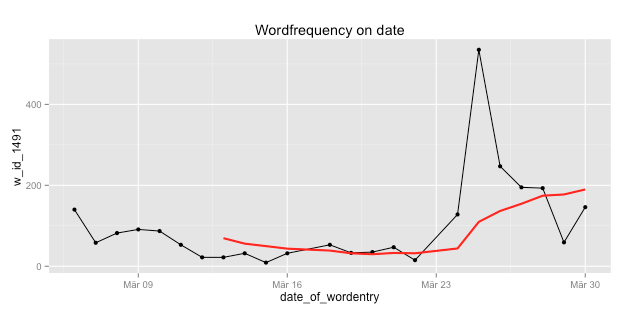
\includegraphics[width=1\textwidth]{pictures/freqratioFlugzeug.png}
	\end{centering}
\end{frame}

\begin{frame}{Relative H\"aufigkeiten - Bemerkungen}
\begin{itemize}
 	\item Erster Ansatz
 	\item Einfache Implementierung
 	\item Selten Auftretende W\"orter werden gegen\"uber anderen interessanten W\"ortern bevorteilt
 \end{itemize}
\end{frame}


\begin{frame}{Poisson als Ma\ss}
	\emph{Idee: } Modellierung der Wahrscheinlichkeit eine bestimmte Frequenz eines Tokens zu sehen. Wenn die Tagesfrequenz eines Tokens sehr unwahrschilich ist, ist das Token interessant.\\
	\emph{Annahme: } Diese Wahrscheinlichkeiten sind Poisson-Verteilt.\\
	\emph{Formel der Poisson-Verteilung allgemein: }
	\begin{equation}
	P_\lambda(k) = \frac{\lambda^{k}}{k!}  \cdot e^{-\lambda}
	\end{equation}
	$\lambda$: Welche Frequenz wird erwartet \\
	(relativer Anteil im Referenzkorpus $\cdot$ Umfang des Tageskorpus)\\
	$k$: tats\"achliches Auftreten von einem Wort k\\
	$P_\lambda(k)$: Erwartete Wahrscheinlichkeit meine Beobachtung k
\end{frame}

\begin{frame}{Poisson-Maß}
% Hier Beispiel Flugzeug
	\hspace{2cm}
	  \begin{centering}
	  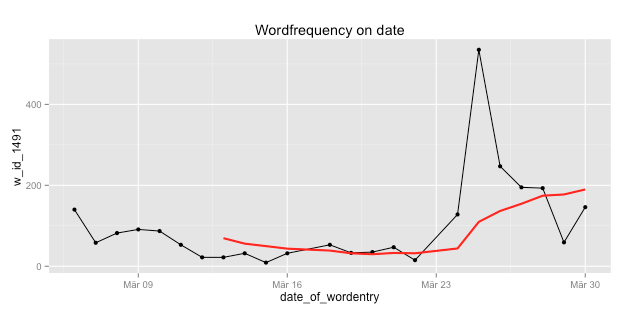
\includegraphics[width=1\textwidth]{pictures/freqratioFlugzeug.png}
	\end{centering}
\end{frame}

\begin{frame}{Poisson als Ma\ss : Implementierung}
	\begin{itemize}
 		\item Problem: Berechnung der Fakult\"at
 		\item Vergleichtbarkeit der Werte einzelner Tage untereinander 
 		\item Ziel: Hoher Rang soll einen hohen Wert haben ($-log$-Methode)
	 \end{itemize}
	 \emph{Formel:}
	 \begin{equation}
		sig_{poisson}(w) = \frac{k(\log(k)-\log(n\cdot p) -1 ))}{\log(n)}
	\end{equation}
\end{frame}

\begin{frame}{Poisson-Verteilung}
% Hier Beispiel Flugzeug 2
	\hspace{1cm}
	  \begin{centering}
	  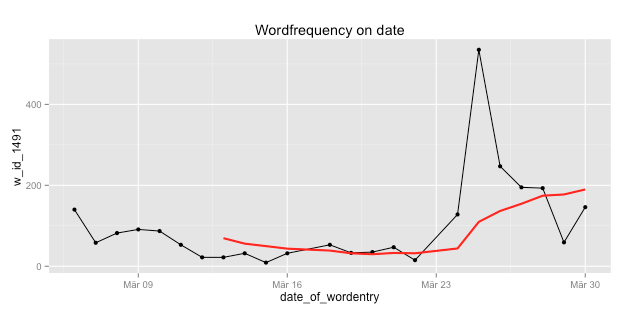
\includegraphics[width=1\textwidth]{pictures/freqratioFlugzeug.png}
	\end{centering}
\end{frame}

\begin{frame}{\emph{Einschub: }\\Wortzahl vs. Satzzahl zur Berechnung relativer Verh\"altnisse}
	\begin{itemize}
		\item{Bei der Referenz wird mit Satzzahlen gearbeitet}
		
		\item{Jeder Satz hat im Schnitt gleiche Anzahl von W\"ortern ($\approx 10$)\\
			\begin{equation}
				\frac{Satz_{heute}}{Satz_{jahr}} \approx \frac{Token_{heute}}{Token_{Jahr}}
			\end {equation}
			}
		\item{Zur \"Uberpr\"ufung sp\"ater mehr}
	\end{itemize}
\end{frame}


\begin{frame}{TF/IDF}
 	\emph{Idee: } Wir gewichten die Auftretensfrequenz eines Token an einem Tag mit dem Inversen einer Maßzahl, die Angibt an wie vielen Tagen im Referenzjahr das Wort erw\"ahnt wurde.\\
	\emph{Modifikationen: } 
	\begin{itemize}
		\item{Relativierung der Frequenz auf Frequenz des h\"aufigsten Tokens am Tag (Vergleichbarkeit)}
		\item{Logarithmieren des IDF-Wertes}
	\end{itemize}
	\emph{Formel:}
	 \begin{equation}
		sig_{tf idf}(w) = \frac{k}{\max(K)} \cdot \log ( \frac{365}{documentdays(w)})
	\end{equation}
	$k$: Frequenz eines Tokens an einem Tag
	$K$: Alle Frequenzen an einem Tag
\end{frame}

\begin{frame}{TF-IDF Beispiel}
% Hier Beispiel Flugzeug 2
	\hspace{1cm}
	  \begin{centering}
	  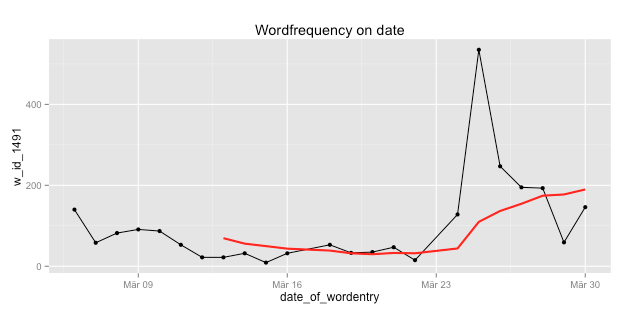
\includegraphics[width=1\textwidth]{pictures/freqratioFlugzeug.png}
	\end{centering}
\end{frame}



\begin{frame}{Z-Score}
	Something about Z-score
\end{frame}

\begin{frame}{Zeitreihenanalyse}
 \begin{definition}[Zeitreihenanalyse]
 	Unter einer Zeitreihe
	versteht man die Entwicklung einer bestimmten Größe, deren Werte im Zeitablauf zu bestimmten Zeitpunkten oder für bestimmte Zeitintervalle erfasst und dargestellt
	werden
 \end{definition}
	
\end{frame}

\begin{frame}{Maß: gleitender Mittelwert}
	\begin{itemize}
		\item Glättet Zeit oder Datenreihen
		\item Erfolgt durch glätten hoher Frequenzanteile
		\item Es gibt ein Raster der größe n		
		\item Es werden n Tage zusammenaddiert und dann durch n geteilt
	\end{itemize}
	
	Wie hilft uns das weiter?
	
	\begin{itemize}
		\item Tritt ein Wort häufiger als sein Durchschnittswert an dem Tag auf kann das interessant sein.
	\end{itemize}		
	
\end{frame}

\begin{frame}{Erster Ansatz: R}
	\begin{itemize}
		\item Der erste Ansatz war ein R Programm welches den gleitenden Mittelwert ausrechnen sollte
		\item Problem: R verarbeitet Wörter einzeln 
		\item 3 Mio. Wörter $\rightarrow$ 3 Mio. Transaktionen = MySQL Overkill
		\item Ausführungszeit würde mehrere Tage beanspruchen
	\end{itemize}
\end{frame}

\begin{frame}{Beispiel}
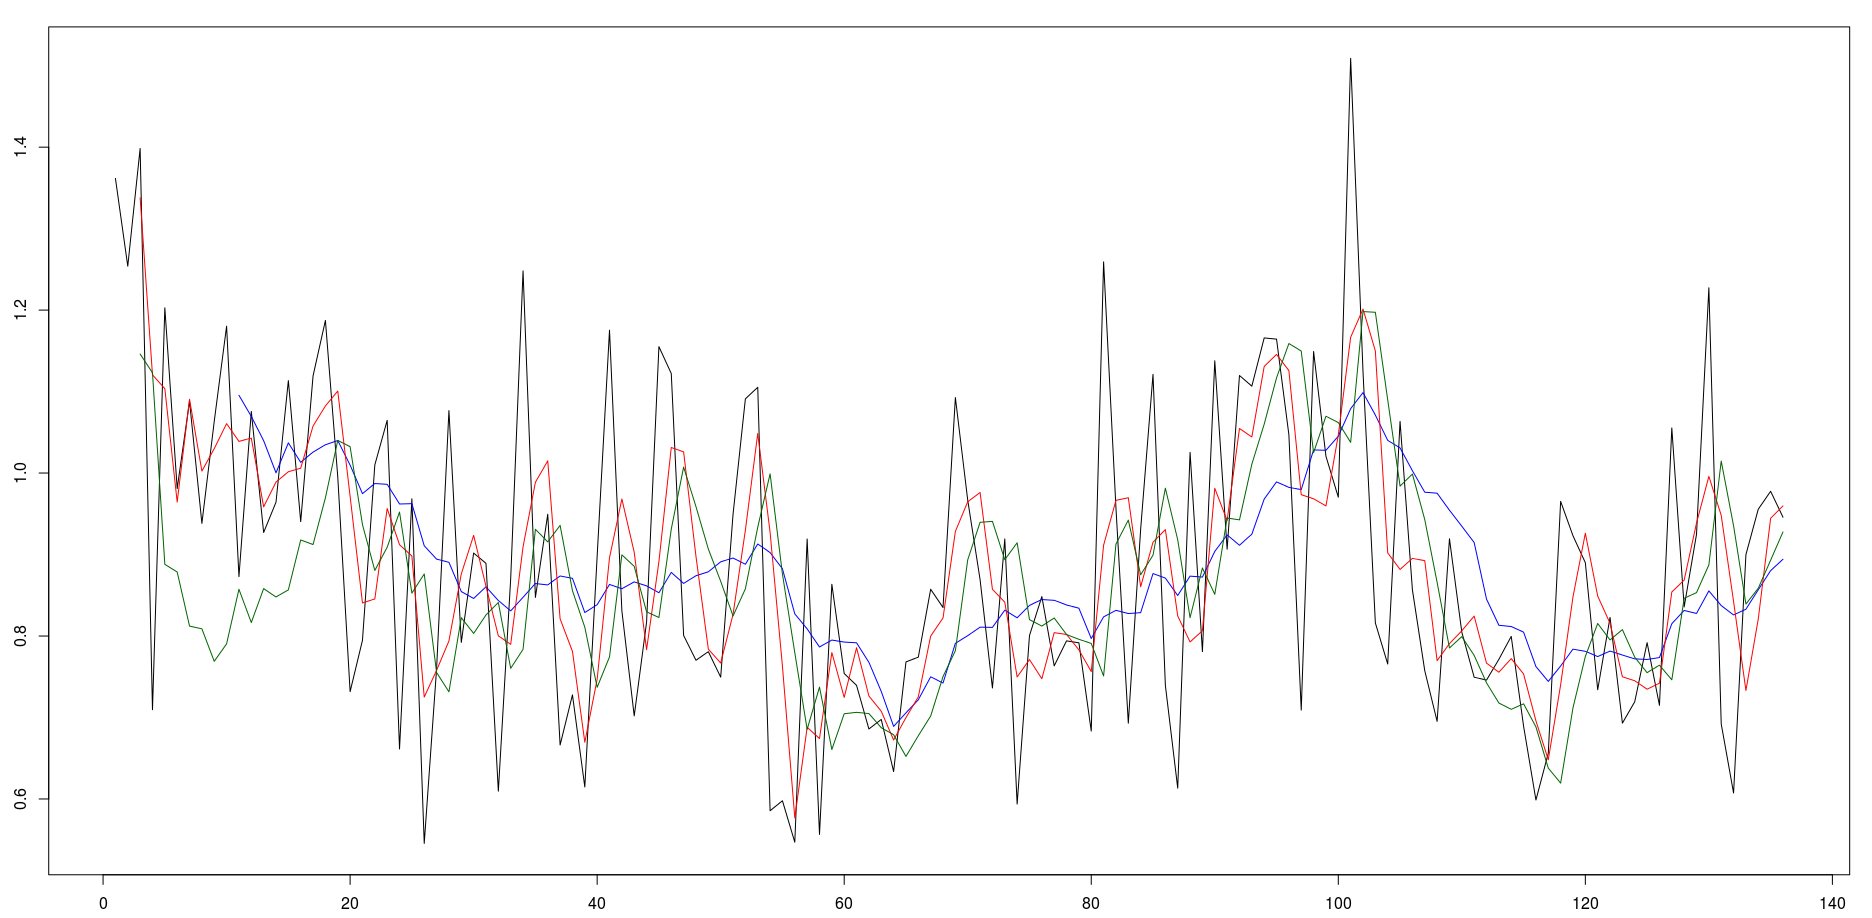
\includegraphics[scale=0.18]{Bilder/R.png}
\end{frame}

\begin{frame}{Zweiter Ansatz: MySQL}
	\begin{itemize}
		\item Der Zweite Ansatz ist es direkt in MySQL zu berechnen
		\item Problem: Inner Join auf selbe Tabelle (ca. 20 Mio Zeilen)
		\item Jeder Eintrag muss geprüft werden ob die Join Tabelle den Eintrag in der Größe des Rasters hat
		\item Eine Datums Differenz Tabelle kann das ganze jedoch beschleunigen

	\end{itemize}
\end{frame}

\section{Vergleich und Auswertung}
\begin{frame} \sectionpage \end{frame}
\begin{frame}{Qualitative vs. Quantitative Auswertung}
	\begin{itemize}
		\item{Schwierigkeit einer quantifizierbaren qualitativen Evaluierung}
		\item{Quantitative vergleiche m\"oglich, aber keine Aussage \"uber Qualit\"at}
		\item{Im Rahmen des Projektes m\"oglich:
			\begin{itemize}
				\item{\emph{``Evaluierung durch draufschauen''}}
				\item{Geeignetes Maß zum quantitativen Verlgeich nutzen}
			\end{itemize}
		}
	\end{itemize}
% Hier Beispiel Flugzeug 2
\end{frame}

\begin{frame}{Qualitative Auswertung}
% Hier Beispiel Flugzeug 2
Hier Beispiellisten f\"ur den 25.3.2015 einf\"ugen.
\end{frame}

\begin{frame}{Quantitative Auswertung}
	\emph{Problemstellung: }Vergleich von sortierten Listen mit potentiell unterschiedlichem Inhalt.
	\begin{itemize}
		\item{Der Vergleich von Wortpaaren nicht sauber m\"oglich.}
		\item{Schwierigkeit eines Mengenbasierter Ansatzes:\\Reihenfolge wird nicht beachtet }
	\end{itemize}	
\end{frame}


\begin{frame}{Quantitative Auswertung: Maximum Overlap}
	\emph{Idee: } Es wird ein Mengenbasierter Ansatz f\"ur Teillisten genutzt und dann gemittelt.\\
	F\"ur jeden Rang der Listen wird eine Teilliste (Rang 1 bis betrachteter Rang) verglichen.\\
	\vspace{1cm}
	\emph{Beispiel:} Tafelbild
\end{frame}

\begin{frame}{Quantitative Auswertung: Maximum Overlap Ergebnisse}
	Tabelle
\end{frame}

\begin{frame}{Quantitative Auswertung: Maximum Overlap Ergebnisse}
	Graph
\end{frame}

\begin{frame}{\emph{Einschub II: }Wortzahl vs. Satzzahl zur Berechnung relativer Verh\"altnisse}
	Graph
	\begin{itemize}
		\item{\"Ubereinstimmung von numerisch 100 Prozent}
	\end{itemize}
\end{frame}



\begin{frame}{Zusammenfassung}
	\begin{itemize}
		\item{Es wurden bestehende Verfahren untersucht}
		\item{Es wurden weitere Verfahren ausprobiert}
		\item{Es wurden die Ergebnisse quantitativ und qualitativ verglichen}
		\item{Es wurden MySQL und R Implementierungen umgesetzt.}
		\item{Es werden noch Musterbasierte Verfahren zum Cleaning der Listen implementiert}
		\item{Es wird noch ein weiteres Verlgleichsmaß mit Ber\"ucksichtigung der Anzahl der Quellen in denen ein Token erw\"ahnt wird untersucht.}
	\end{itemize}
\end{frame}



\begin{frame}[allowframebreaks]{Quellen}
	\nocite{*}
	\bibliographystyle{plaindin}
    \bibliography{quellen}
\end{frame}

\end{document}

